\documentclass[twocolumn]{article}

\usepackage{imr}
\usepackage{graphicx}
\usepackage{amsfonts}
\usepackage{bbm}       % for \mathbbm{1}
\usepackage{amsmath}
\usepackage{mathrsfs}  % for \mathscr
\usepackage{minted}    % for including source code
\usepackage{tikz}
\usetikzlibrary{decorations.markings}

\def\thepage {}
\bibliographystyle{imr}

\newenvironment{smallarray}[1]
 {\null\,\vcenter\bgroup\scriptsize
  \renewcommand{\arraystretch}{0.7}%
  \arraycolsep=.13885em
  \hbox\bgroup$\array{@{}#1@{}}}
 {\endarray$\egroup\egroup\,\null}

\begin{document}

\title{Linear-algebraic representation and transformation of unstructured meshes}
\author{Daniel Shapero$^1$}
\date{
    $^1$University of Washington, Seattle, WA, USA, shapero@uw.edu
}

\abstract{This paper will show some new approaches for implementing common transformations to the connectivity or topology of an unstructured mesh.
The key enabling technology for our approach is to borrow ideas from algebraic topology: we use the \emph{boundary operators} of a \emph{chain complex} to represent the mesh.
Boundary operators are really just integer matrices.
By representing the objects of study using the language of linear algebra, we can use linear algebraic reasoning and intuition to define transformations.}

\keywords{mesh generation, computational geometry, algebraic topology}

\maketitle
\thispagestyle{empty}
\pagestyle{empty}


% --------------------
\section{Introduction}

In this paper, we'll explore some of the computational kernels for unstructured meshing.
Nearly all problems in meshing require the ability to perform local transformations to the mesh topology.
For example, to compute the Delaunay triangulation, the Lawson algorithm uses a sequence of bistellar flips, while the Bowyer-Watson algorithm is based on splitting star-shaped polytopes along a vertex \cite{cheng2013delaunay}.
Algorithms for mesh coarsening, on the other hand, apply a sequence of edge or face collapses \cite{cignoni1998comparison}.
Implementing these low-level transformation kernels on common mesh data structures can be difficult and error-prone.
Are there other mesh data structures that make common algorithms easier to implement?

The idea of \emph{linear-algebraic representation} is to describe the mesh topology using a sequence of linear operators between certain vector spaces or modules.
The linear algebraic representation of meshes comes from algebraic topology: the \emph{boundary operators} on a certain \emph{chain complex}.
\textbf{If we can describe the mesh topology using linear algebra, then we can transform it using linear algebra as well.}
This viewpoint has been adopted in several publications on meshing and solid modeling \cite{dicarlo2007solid}, \cite{dicarlo2014linear}, \cite{mueller2017ternary}, \cite{paoluzzi2020topological}.
Other domains of science and engineering have seized on the idea of using linear algebra as the common language for building applications as well.
For example, the GraphBLAS project aims to implement common algorithms in graph theory using linear algebra \cite{mattson2013standards}.

In \textcolor{red}{Shapero (2023)}, I showed how to implement two transformations -- splitting a cell on a vertex and merging adjacent cells -- on the linear-algebraic representation of a polygonal mesh.
I then demonstrated how to compute convex hulls and Delaunay triangulations in higher dimensions using these kernels.
The main advantage of this linear-algebraic approach is that the transformation kernels are easy to write down and to code.
Our contribution here is an extension of this work to an additional transformation: splitting a cell on a collection of facets.
This transformation can also be expressed entirely with linear algebra.
We provide a proof-of-concept application to computed constrained Delaunay meshes and 2D and 3D.


% --------------
\section{Theory}

In this section, we'll describe some of the mathematical theory that underlies the constructions that follow.
Understanding this theory at a profound level isn't strictly necessary in order to understand how we instrumentalize it to perform computations.
But our objects of study are more abstract than, say, a simplex or other point set.
A point set can be described solely through what its members are; the objects we are interested in carry with them an additional notion of orientation.

As we alluded to before, the underlying theory is basic algebraic topology.
The usual introduction to algebraic topology starts with CW complexes \cite{hatcher2002algebraic}.
But understanding how to get from a CW complex to what we really care about -- a sequence of boundary operators -- requires some advance knowledge of homology or degree theory first.
Moreover, these boundary operators are linear mappings between certain modules, the spaces of \emph{chains}.
The chain spaces are defined as formal linear combinations of cells of the mesh.
On introducing the idea of chains, many readers will scratch their heads and wonder what on earth we mean by multiplying a triangle by four -- is it creating four copies of a triangle?
Not quite...
In our experience, readers find it unsatisfying to hand-wave the issue away by telling them to think of these algebraic operations as purely formal manipulations with no intrinsic meaning.

Instead, we will take as our theoretical underpinning the theory of \emph{currents} on a manifold.
The theory of currents is a kind of dual to the theory of differential forms.
The main advantage is that it gives a clear concept for what it means to multiply a submanifold by an integer or even a real number.

\subsection{Differential forms}

Let $\Omega$ be a compact, orientable manifold, and $u$ a completely antisymmetric tensor field of rank $k$ on $\Omega$.
Such a tensor field is called a \emph{differential $k$-form}.
We will write the space of all $k$-forms by $\mathscr{F}_k(\Omega)$ or just $\mathscr{F}_k$ when the underlying manifold is clear from context.

Given a $k$-form $u$ and an $\ell$-form $v$, we can form their \emph{wedge} or \emph{exterior} product $u \wedge v$, which is a $(k + \ell)$-form.
The wedge product is obtained by anti-symmetrizing the outer product of the two forms.

The \emph{exterior derivative} on forms $d_k$ is a differential operator which takes in a $k$-form and gives a $(k + 1)$-form.
Where the rank $k$ of the form can be determined from context, we'll write $d$ and leave off the subscript.
The exterior derivative can be defined axiomatically by requiring that (1) if $f$ is a scalar field or 0-form, then its exterior derivative is equal to its differential; (2) if $f$ is a scalar field, then $d(df) = 0$; and (3) $d(u \wedge v) = du\wedge v + (-1)^k u \wedge dv$.
From these properties, we can deduce that $d(du) = 0$ for any form $u$.

Most important for us is the generalized \emph{Stokes theorem}.
Given a $k$-form $u$ and an oriented $k$-dimensional submanifold $M$, we can define the integral of $u$ on $M$.
The generalized Stokes theorem states that, for a $k - 1$-form $u$,
\begin{equation}
    \int_Mdu = \int_{\partial M}u.
\end{equation}
This includes Green's theorem, the divergence theorem, and the classical Stokes theorem as special cases.

\subsection{Currents}

A $k$-\emph{current} is a continuous linear functional from the space of $k$-forms $\mathscr{F}_k(\Omega)$ to the reals.
We denote the action of a current $J$ on a form $u$ by $\langle J, u\rangle$ and the space of all $k$-currents by $\mathscr{C}^k(\Omega)$.
The space of $k$-currents naturally has the structure of a vector space.
Currents are exactly analogous to spaces of distributions as defined in PDE theory, but with the extra tensorial character of differential forms.

We can think of an oriented submanifold $M$ as defining a $k$-current by integration:
\begin{equation}
    \langle M, u\rangle \equiv \int_M u.
\end{equation}
(Here we'll abuse notation a little bit by writing both the oriented submanifold and the linear functional as ``$M$''.
Some texts opt to use a different notation for the current induced by a submanifold to disambiguate between the two but this level of detail won't be necessary.)
Not all currents are definable by integration over a submanifold.
For example, given a point $x$ and a vector $\xi$ in the tangent space to $\Omega$ at $x$, the mapping $f \mapsto df(x)\cdot\xi$ is a well-defined 0-current, but it is not definable by integration.
A current $J$ is called \emph{rectifiable} if
\begin{equation}
    \langle J, u\rangle = \alpha\int_Mu
\end{equation}
for some integer $\alpha$ and some oriented submanifold $M$ with finite Hausdorff measure.
Note that the current $-M$ represents integration over $M$ if we give it the opposite orientation.

Given two submanifolds $M$ and $N$ of the same dimension and real numbers $\alpha$ and $\beta$, we can define their linear combination $\alpha \cdot M + \beta\cdot N$ by how this current acts on forms.
A linear combination of currents need not be definable as integration over some oriented submanifold, even when the summands are; again, all that matters is how the sum acts on forms.

Now we can define the \emph{boundary} $\partial_k J$ of a $k$-current $J$ as the formal adjoint of the exterior derivative $d_{k - 1}$:
\begin{equation}
    \langle\partial_k J, u\rangle \equiv \langle J, d_{k - 1}u\rangle.
\end{equation}
Once again, when the dimension $k$ of the current is clear from context, we will write just $\partial$ and drop the subscript.
When $J$ is integration over an oriented submanifold, this definition agrees with the generalized Stokes theorem.
We say that $J$ is an \emph{integral} current if both $J$ and $\partial J$ are rectifiable.

The boundary operator is a linear map from $\mathscr{C}^k$ to $\mathscr{C}^{k - 1}$.
Since $d(du) = 0$ for any differential form $u$, we can then show that $\partial(\partial J) = 0$.
This equation is more commonly expressed purely in terms of the boundary operators as
\begin{equation}
    \partial_k\cdot\partial_{k + 1} = 0.
    \label{eq:ddzero}
\end{equation}
and this is the most important property of boundary operators.
Moreover, equation \eqref{eq:ddzero} implies that the spaces $\{\mathscr{C}^k\}$ together with the mappings $\partial_k : \mathscr{C}^k \to \mathscr{C}^{k - 1}$ are a \emph{chain complex}.

There is one final definition that will clarify a later construction at a critical juncture.
The definitions above assume that the chain complex terminates at $\mathscr{C}^0$, i.e. continuous linear functionals on the space of scalar fields.
We will instead include a \emph{bottom} space $\mathscr{C}^{-1}$ which is isomorphic to $\mathbb{R}$.
We then wish to define a 0-boundary operator $\partial_0 : \mathscr{C}^0 \to \mathbb{R}$ such that $\partial_0\partial_1 = 0$.
Remembering that the 0-currents are continuous linear functionals on the space of scalar fields, we will define the 0-boundary operator as follows:
\begin{equation}
    \partial_0 J = \langle J, 1\rangle,
    \label{eq:0-boundary-operator}
\end{equation}
i.e. take the action of $J$ on the constant function $u(x) = 1$.
For example, if $J$ is a rectifiable 0-current, then $J$ must have the form
\begin{equation}
    J = \sum_ia_i\delta_{x_i}
\end{equation}
for some finite collection of points $\{x_i\}$.
Then
\begin{equation}
    \partial_0J = \sum_i a_i.
\end{equation}
Requiring that $\partial_0\partial_1 = 0$ then implies, for example, that rectifiable 1-currents have to be a sum of circles or curves that goes from one point to another point.
\textcolor{red}{I want to talk about incidence numbers between currents here but we haven't introduced that concept yet.}

\subsection{Meshes}

We can now define a mesh in terms of currents on some background manifold $\Omega$ of dimension $n$.
An unstructured mesh is a collection $\{C^0, \ldots, C^n\}$ of finite-dimensional submodules of the integral $k$-currents that are closed under taking boundaries.
In other words, for any current $M$ in $C^k$,
\begin{equation}
    \partial_k M = \sum_ic_iN_i
\end{equation}
where $N_i$ are all in $C^{k - 1}$ and the coefficients $c_i$ are all integers.
With a slight abuse of notation, we will use $\partial_k$ to denote the restriction of the boundary operator as a linear map $\partial_k : C^k \to C^{k - 1}$.
This definition has one main advantage over the conventional definition of an abstract simplicial complex.
The $\mathbb{Z}$-module structure of the spaces of integral currents naturally accounts for orientations in a way that needs to be bolted on after the fact for simplicial complexes.

Once we have chosen bases for the vector spaces $C^k$ and $C^{k - 1}$, we can represent the boundary operator $\partial_k$ as a matrix with integer entries.
These sparse integer matrices are the data structure that we will use to describe meshes and which we will perform transformations on.
The condition \eqref{eq:ddzero} is an invariant of this data structure, and preservation of this invariant is a strong constraint on any transformations that we might define.

Having restricted ourselves to finite-dimensional subspaces of the full chain spaces, the matrix that represents the 0-boundary operator is the row vector of all 1s:
\begin{equation}
    \partial_0 = \mathbbm{1}^*.
    \label{eq:0-boundary-matrix}
\end{equation}
At a linear algebraic level, the condition that $\partial_0\partial_1 = 0$ now forces every column of $\partial_1$ to sum of up to zero.
The desired behavior is that every 1-current or edge of the mesh has a single -1 entry and a single +1 entry in the corresponding column of $\partial_1$, although strictly speaking no condition enforces this behavior exactly.
This equation will reappear when we define the split transformation.


% -----------------------
\section{Transformations}

Here we will describe three different transformations that are easily implementable on the linear-algebraic representation of a mesh.
A \textbf{merge} operation combines several adjacent cells into one cell.
A \textbf{split} subdivides a cell into several cells along a new vertex.
A \textbf{bisection} subdivides a cell into two along a new facet.
The merge and split operations have appeared in \textcolor{red}{Shapero (2023)}, but we repeat them here for completeness.
The bisection operation is new.

Before showing the transformations themselves, it's worth considering some of the transformations of a chain complex that leave it unaltered.
First, observe that if $A$, $B$ are integer matrices such that the image of $\partial_{k + 1}$ is an invariant subspace of $A\cdot B$, then the matrices
\begin{equation}
    \partial_k' = \partial_k\cdot A, \quad \partial_{k + 1}' = B\cdot\partial_{k + 1}
\end{equation}
still satisfy $\partial_k'\cdot\partial_{k + 1}' = 0$.
A particular case is $A\cdot B = I$, which includes permutations of the cell ordering.
The more general case regarding the image of $A\cdot B$ is needed for some irreversible transformations.

\subsection{Merging}

A \emph{merge} of a set of $k$-cells replaces them with a single cell (provided that their union is simply-connected).
Merging is a column operation on the matrix $\partial_k$.
In the simplest case, the result column is the sum of all the columns to be merged, but in general we might need to flip some signs:
\begin{align}
    \partial_k' & = \partial_k\cdot\text{diag}(s_0, \ldots, s_m)\cdot\mathbbm{1}, \\
    \partial_{k + 1}' & = \left[\begin{matrix} 0 \ldots 1 \ldots 0\end{matrix}\right]\partial_{k + 1}. \label{eq:merge-k+1}
\end{align}
where $s_i$ are all $\pm 1$.
The signs are chosen so that any higher-dimensional cell $\sigma$ has the same incidence with respect to any of the cells $\tau$ to be merged.
The transformation to the rows of $\partial_{k + 1}$ collapses all incidence to any of the desired $k$-cells into incidence to the merged $k$-cell.
For merging cells of top dimension $n$, there are no higher-dimensional cells to apply equation \eqref{eq:merge-k+1} to and this step is left out.

\emph{Edge collapsing}, the key transformation in surface simplification algorithms \cite{gueziec1995surface}, is a merge of two vertices.


\subsection{Splitting}

A \emph{split} divides up the union of several polytopes along a vertex.
The key correctness criteria for this operation are that (1) every newly-created polytope contains the splitting vertex and (2) the boundary of the sum of all polytopes does not change.
This second condition can be expressed mathematically as
\begin{equation}
    \partial_k'\mathbbm{1} = \left[\begin{matrix}\partial_k\mathbbm{1} \\ 0\end{matrix}\right].
    \label{eq:split-preserves-boundaries}
\end{equation}
We'll describe the 2D case first and then proceed to arbitrary dimensions.

Suppose that a collection of adjacent polygons has the boundary operators $\partial_1$ and $\partial_2$.
We first have to draw edges between the new vertex and all the vertices of the polygon.
The orientation of these new edges is arbitrary, so we can assume that every edge goes from the splitting vertex $v$ to the polygon vertices.
Another way of stating this is that every new edge $e$ is negatively-incident to $v$ and positively-incident to some polygon vertex.
In terms of matrices, the new 1-boundary operator is
\begin{equation}
    \partial_1' = \left[\begin{matrix}\partial_1 & I \\ 0 & -\mathbbm{1}^*\end{matrix}\right]
    \label{eq:split-1-2d}
\end{equation}
where $I$ is the identity matrix.
The key step here is defining the 2-boundary matrix:
\begin{equation}
    \partial_2' = \left[\begin{matrix}\text{diag}(\partial_2\cdot\mathbbm{1}) \\ -\partial_1\cdot\text{diag}(\partial_2\cdot\mathbbm{1})\end{matrix}\right]
\end{equation}
A rudimentary calculation shows that $\partial_1'\partial_2' = 0$.
Since $\text{diag}(z)\cdot\mathbbm{1} = z$ for any vector $z$, we also find that
\begin{equation}
    \partial_2'\mathbbm{1} = \left[\begin{matrix}\partial_2\mathbbm{1} \\ 0\end{matrix}\right]
\end{equation}
which is exactly equation \eqref{eq:split-preserves-boundaries}, or that the new polygons have the same boundary as the old.
Figure \ref{fig:split-transformation} illustrates the split transformation on a single quadrilateral and shows the boundary matrices before and after.

\begin{figure}[h]
    \begin{center}
        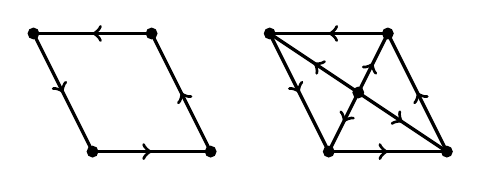
\begin{tikzpicture}[scale=0.75]
            \newcommand*{\defcoords}{
                \coordinate (p0) at (1.5, 1){};
                \coordinate (p1) at (1, 0){};
                \coordinate (p2) at (3, 0){};
                \coordinate (p3) at (2, 2){};
                \coordinate (p4) at (0, 2){};
            }

            \begin{scope}[
                very thick,
                decoration={markings, mark=at position 0.5 with {\arrow{>}}}
            ]
                \defcoords
                \draw[postaction={decorate}] (p1) -- (p2);
                \draw[postaction={decorate}] (p2) -- (p3);
                \draw[postaction={decorate}] (p3) -- (p4);
                \draw[postaction={decorate}] (p4) -- (p1);

                \foreach \p in {p1, p2, p3, p4} {
                    \filldraw (\p) circle (2pt);
                }
            \end{scope}

            \begin{scope}[
                very thick,
                shift={(4, 0)},
                decoration={markings, mark=at position 0.5 with {\arrow{>}}}
            ]
                \defcoords
                \draw[postaction={decorate}] (p1) -- (p2);
                \draw[postaction={decorate}] (p2) -- (p3);
                \draw[postaction={decorate}] (p3) -- (p4);
                \draw[postaction={decorate}] (p4) -- (p1);
                \draw[postaction={decorate}] (p0) -- (p2);
                \draw[postaction={decorate}] (p0) -- (p3);
                \draw[postaction={decorate}] (p0) -- (p4);
                \draw[postaction={decorate}] (p0) -- (p1);

                \foreach \p in {p0, p1, p2, p3, p4} {
                    \filldraw (\p) circle (2pt);
                }
            \end{scope}
        \end{tikzpicture}
    \end{center}

    \begin{equation*}
        \partial_1 = \left[\begin{smallmatrix}
            - &   &   & + \\
            + & - &   &   \\
              & + & - &   \\
              &   & + & -
        \end{smallmatrix}\right],
        \quad
        \partial_2 = \left[\begin{smallmatrix}
            + \\ + \\ + \\ +
        \end{smallmatrix}\right]
    \end{equation*}

    \begin{equation*}
        \partial_1' = \left[\begin{smallarray}{cccc|cccc}
            - &   &   & + & + &   &   &   \\
            + & - &   &   &   & + &   &   \\
              & + & - &   &   &   & + &   \\
              &   & + & - &   &   &   & + \\
            \hline
              &   &   &   & - & - & - & -
        \end{smallarray}\right], \quad
        \partial_2' = \left[\begin{smallarray}{cccc}
            + &   &   &   \\
              & + &   &   \\
              &   & + &   \\
              &   &   & + \\
            \hline
            + &   &   & - \\
            - & + &   &   \\
              & - & + &   \\
              &   & - & +
        \end{smallarray}\right]
    \end{equation*}

    \caption{Quadrilateral before and after splitting on a new vertex in the center (top) and boundary matrices before and after (bottom).}
    \label{fig:split-transformation}
\end{figure}

We can get an idea for how to extend this to $n$ dimensions by remembering the 0-boundary operator (equation \eqref{eq:0-boundary-matrix}).
In equation \eqref{eq:split-1-2d}, we can replace $\mathbbm{1}^* = \partial_0$.
This suggests the transformation
\begin{align}
    \partial_k' & = \left[\begin{matrix}\partial_k & I \\ 0 & -\partial_{k - 1}\end{matrix}\right] \label{eq:split-k} \\
    \partial_n' & = \left[\begin{matrix}\text{diag}(\partial_n\cdot\mathbbm{1}) \\ -\partial_{n - 1}\text{diag}(\partial_n\cdot\mathbbm{1})\end{matrix}\right] \label{eq:split-n}
\end{align}
Again, a rudimentary calculation shows that the fundamental equation \eqref{eq:ddzero} still holds and that the new polytopes have the same boundary as the old.

Equation \eqref{eq:split-k} has appeared before in the literature on homological algebra as the expression for the boundary operators of the \emph{cone} of a space \cite{gelfand1994homological}.
To our knowledge, using these equations for doing real computations is entirely new.

The Bowyer-Watson algorithm for Delaunay triangulation and all common algorithms for computing convex hulls only require the split transformation \cite{cheng2013delaunay}.

\subsection{Splitting and merging}

Other transformations can be defined by combining a sequence of splits and merges.
For example, figure \ref{fig:2-2-flip} shows how to perform a 2-2 flip in 2D by first splitting the quadrilateral into four triangles and then performing a sequence of merges and figure \ref{fig:2-3-flip} shows the same process for a 2-3 flip in 3D.
(We've shown an initial merge step for illustrative purposes, but this merge is actually part of the subsequent split.)

\begin{figure}[h]
    \tikzset{ec/.style={every coordinate/.try}}

    \begin{center}
    \begin{tikzpicture}[scale=0.4]
        \coordinate (p0) at (1.5, 1){};
        \coordinate (p1) at (1, 0){};
        \coordinate (p2) at (3, 0){};
        \coordinate (p3) at (2, 2){};
        \coordinate (p4) at (0, 2){};

        \begin{scope}[very thick]
            \draw (p1) -- (p2) -- (p4) -- cycle;
            \draw (p4) -- (p3) -- (p2) -- cycle;

            \foreach \p in {p1, p2, p3, p4} {
                \filldraw (\p) circle (3pt);
            }
        \end{scope}

        \begin{scope}[very thick, every coordinate/.style={shift={(3.5,0)}}]
            \draw ([ec]p1) -- ([ec]p2) -- ([ec]p3) -- ([ec]p4) -- cycle;

            \foreach \p in {p1, p2, p3, p4} {
                \filldraw ([ec]\p) circle (3pt);
            }
        \end{scope}

        \begin{scope}[very thick, every coordinate/.style={shift={(7,0)}}]
            \draw ([ec]p0) -- ([ec]p1) -- ([ec]p2) -- cycle;
            \draw ([ec]p0) -- ([ec]p2) -- ([ec]p3) -- cycle;
            \draw ([ec]p0) -- ([ec]p3) -- ([ec]p4) -- cycle;
            \draw ([ec]p0) -- ([ec]p4) -- ([ec]p1) -- cycle;

            \foreach \p in {p0, p1, p2, p3, p4} {
                \filldraw ([ec]\p) circle (3pt);
            }
        \end{scope}

        \begin{scope}[very thick, every coordinate/.style={shift={(10.5,0)}}]
            \draw ([ec]p1) -- ([ec]p2) -- ([ec]p3) -- cycle;
            \draw ([ec]p3) -- ([ec]p4) -- ([ec]p1) -- cycle;

            \foreach \p in {p0, p1, p2, p3, p4} {
                \filldraw ([ec]\p) circle (3pt);
            }
        \end{scope}

        \begin{scope}[very thick, every coordinate/.style={shift={(14,0)}}]
            \draw ([ec]p1) -- ([ec]p2) -- ([ec]p3) -- cycle;
            \draw ([ec]p3) -- ([ec]p4) -- ([ec]p1) -- cycle;

            \foreach \p in {p1, p2, p3, p4} {
                \filldraw ([ec]\p) circle (3pt);
            }
        \end{scope}

        \begin{scope}[very thick]
            \draw[->] (2, -0.2) arc[start angle=180, end angle=360, radius=1.5] node[midway, below, align=center] {merge\\triangles};
            \draw[->] (5.5, -0.2) arc[start angle=180, end angle=360, radius=1.5] node[midway, below] {split};
            \draw[->] (9.0, -0.2) arc[start angle=180, end angle=360, radius=1.5] node[midway, below, align=center] {merge\\triangles};
            \draw[->] (12.5, -0.2) arc[start angle=180, end angle=360, radius=1.5] node[midway, below, align=center] {merge\\edges};
        \end{scope}
    \end{tikzpicture}
    \end{center}
    \caption{A 2-2 flip, implemented as a sequence of merges and splits.
    The vertex added by splitting the quadrilateral is deleted when the two edges are merged in the final transformation.}
    \label{fig:2-2-flip}
\end{figure}

\begin{figure}[h]
    \begin{center}
        \input{figures/tetrahedra.tikz}
    \end{center}
    \caption{A 2-3 flip implemented as a sequence of merges and splits.
    We've shown the tetrahedra in an ``exploded'' view to help with visualization.}
    \label{fig:2-3-flip}
\end{figure}

\textcolor{red}{This text is copied over from the short paper but it needs revisiting.
The current paper is supposed to do or at least enable multi-face retriangulation so we need to be less speculative and prove the concept.}
A few papers have proposed using multi-cell transformations for 3D mesh improvement \cite{klingner2008aggressive}.
Multi-cell transformations are more complex than 2-3 or 3-2 flips, but \cite{misztal2009tetrahedral} showed that they can be implemented as a sequence of flips.
Using the boundary operators might make it possible to implement complex transformations with less effort.
The split transformation that we derived here is based on computing the topological cone of a space and then removing the base of the cone.
Multiface retriangulation, as advocated in \cite{misztal2009tetrahedral}, is a transformation of a \emph{suspension}, a related construction in algebraic topology \cite{hatcher2002algebraic}.

\subsection{Bisection}

Finally, we consider the problem of how to split a single $k$-cell in two along some $(k - 1)$-cell.
We first consider the structure of the cell we wish to split.
The boundary matrices must first have the form
\begin{equation}
    \partial_k = \left[\begin{matrix}[V_1, E_1] & 0 \\ 0 & [V_2, E_2] \\ [V_3, E_1] & [V_3, E_2]\end{matrix}\right], \quad \partial_{k + 1} = \left[\begin{matrix}[E_1, T] \\ [E_2, T]\end{matrix}\right].
\end{equation}
The condition that $\partial_k\cdot\partial_{k + 1} = 0$ gives us several identities to work with:
\begin{align}
    [V_1, E_1][E_1, T] & = 0 \\
    [V_2, E_2][E_2, T] & = 0 \\
    [V_3, E_1][E_1, T] + [V_3, E_2][E_2, T] & = 0 \label{eq:bisect-start}
\end{align}
Now we want to split the cell $T$ into two cells $T_1$ and $T_2$ such that $T = T_1 + T_2$.
The new boundary matrices will have the form
\begin{align}
    & \partial_k' = \left[\begin{matrix}[V_1, E_1] & 0 & 0 \\ 0 & [V_2, E_2] & 0 \\ [V_3, E_1] & [V_3, E_2] & [V_3, E_3] \end{matrix}\right], \\
    & \quad \partial_{k + 1}' = \left[\begin{matrix}[E_1, T_1] & 0 \\ 0 & [E_2, T_2] \\ [E_3, T_1] & [E_3, T_2]\end{matrix}\right]
\end{align}
We can make a few simplifications right away by requiring that merging $T_1$ and $T_2$ back into a single cell will give back the original complex.
Formally, this means that
\begin{equation}
    \partial_{k + 1}'\cdot\left[\begin{matrix} I & I\end{matrix}\right] = \partial_{k + 1}.
\end{equation}
The immediate consequence is that $[E_1, T_1] = [E_1, T]$, $[E_2, T_2] = [E_2, T]$ and
\begin{equation}
    [E_3, T_1] + [E_3, T_2] = 0.
\end{equation}
We will then introduce the unknown matrix $[E_3, T]$ and define $[E_3, T_1] = [E_3, T]$, $[E_3, T_2] = -[E_3, T]$.
The remaining conditions to preserve the chain complex property are
\begin{align}
    [V_3, E_1][E_1, T] + [V_3, E_3][E_3, T] & = 0 \\
    [V_3, E_2][E_2, T] - [V_3, E_3][E_3, T] & = 0
\end{align}
In principle, this system might appear to be over-determined, but adding up the two equations gives back equation \eqref{eq:bisect-start}.

\textcolor{red}{Finish this.
I haven't introduced what the $[\cdot,\cdot]$ notation means because in the short version this was the topological degree of the attaching map.
I don't know how this is defined for currents.}


% ---------------------
\section{Demonstration}

As a proof of concept, we developed a software package called \emph{zmsh} which implements the split transformation defined above \cite{shapero2023zmsh}.
The source code for the split transformation is shown in figure \ref{fig:split-source-code}.
\begin{figure}
    \begin{minted}[fontsize=\footnotesize,linenos]{python}
import numpy as np
from typing import List

def split(D: List[np.ndarray]) -> List[np.ndarray]:
    # Create the boundary matrices for 1 <= k < n
    n_vertices = D[0].shape[1]
    E = [np.ones((1, n_vertices + 1), int)]
    for k in range(1, len(D) - 1):
        n_cells = D[k].shape[1]
        n_sub_faces, n_faces = D[k - 1].shape
        I = np.identity(n_faces, int)
        Z = np.zeros((n_sub_faces, n_cells), int)
        E_k = np.block([[D[k], I], [Z, -D[k - 1]]])
        E.append(E_k)

    # Create the top-dimensional boundary matrix
    C = np.diag(np.sum(D[-1], axis=1))
    E_n = np.vstack((C, -D[-2] @ C))
    E.append(E_n)
    return E
    \end{minted}
    \caption{Python source code for the split transformation.
    Line 13 corresponds to equation \eqref{eq:split-k}; lines 17 and 18 correspond to equation \eqref{eq:split-n}.
    The real version has some additional logic to remove empty cells.}
    \label{fig:split-source-code}
\end{figure}
We used the split transformation to implement a convex hull algorithm that works in arbitrary dimensions.
To test the convex hull code, we used (1) random point sets up to dimension 5 and (2) several synthetic input sets with various degeneracies such as coplanarity.
\textcolor{red}{This next sentence was copied over from the short paper, and it was true at the time.
Now we have a package that uses interval arithmetic and falls back to bignum rational, which is much faster.
We should finish testing that, make sure it works for the insphere predicate, and say something about it.}
For geometric predicates, we used the Python standard library's built-in routines to convert a floating point value exactly to a ratio of big integers.


% ------------------
\section{Conclusion}

Doubly-connected edge lists have historically been popular for mesh generation because they offer a simple interface for traversing the topology \cite{guibas1985primitives}.
Here we propose that boundary operators are an ideal representation if the goal is to perform topological transformations.
This idea has appeared before, for example in the work of DiCarlo and others \cite{dicarlo2007solid}.

Boundary operators are only necessary for representing a small patch of the topology at a time.
Once the transformed patch is computed, it can be translated back to a set of simplexes.
Boundary operators are useful for describing non-simplicial intermediate states of a transformation; they are not space-optimal for describing an entire simplicial complex.

When the objects of study can be represented as linear operators, we can apply linear algebraic reasoning to define transformations and verify that they preserve all of the important invariants.
The condition in equation \eqref{eq:ddzero} that the product of two boundary operators is zero is a powerful invariant for ensuring the validity of the underlying topology.


\bibliography{chain-complexes.bib}

\end{document}
